\documentclass[nobib, a4paper]{tufte-book}
\usepackage{microtype, ifluatex, ifxetex}
%Next block avoids bug, from  http://tex.stackexchange.com/a/200725/1913 
\ifx\ifxetex\ifluatex\else % if lua- or xelatex http://tex.stackexchange.com/a/140164/1913
  \usepackage{fontspec}
  \setmainfont[Renderer=Basic, Numbers=OldStyle, Scale = 1.0]{TeX Gyre Pagella}
  \setsansfont[Renderer=Basic, Scale=0.90]{TeX Gyre Heros}
  \setmonofont[Renderer=Basic]{TeX Gyre Cursor}

  \renewcommand{\textls}[2][5]{%
    \begingroup\addfontfeatures{LetterSpace=#1}#2\endgroup
  }
  \renewcommand{\allcapsspacing}[1]{\textls[15]{#1}}
  \renewcommand{\smallcapsspacing}[1]{\textls[10]{#1}}
  \renewcommand{\allcaps}[1]{\textls[15]{\MakeTextUppercase{#1}}}
  \renewcommand{\smallcaps}[1]{\smallcapsspacing{\scshape\MakeTextLowercase{#1}}}
  \renewcommand{\textsc}[1]{\smallcapsspacing{\textsmallcaps{#1}}}
\fi

\usepackage{graphicx} % allow embedded images
  \setkeys{Gin}{width=\linewidth,totalheight=\textheight,keepaspectratio}
  \graphicspath{{images/}} % set of paths to search for images
\usepackage{amsmath,amssymb,amsthm,amsfonts,ulem,tikz}  % extended mathematics
\usepackage{booktabs} % book-quality tables
\usepackage{units}    % non-stacked fractions and better unit spacing
\usepackage{multicol} % multiple column layout facilities
\usepackage{fancyvrb,xcolor} % extended verbatim environments
  \fvset{fontsize=\normalsize}% default font size for fancy-verbatim environments
\usepackage{tikz-cd,bbm,mathbbol}
\DeclareSymbolFontAlphabet{\mathbbl}{bbold} %let's you use \mathbbl{k} for a field k
\hypersetup{colorlinks} %puts color to hyperlinks
\setcounter{secnumdepth}{2} 
\usepackage{enumerate}
\usepackage{mathabx}
\usepackage{mathtools}
\usepackage{nccmath}
\usepackage[english]{babel}
\usepackage{hyperref}
\hypersetup{
    colorlinks=true,    
    urlcolor=Cerulean,
    linkcolor = ForestGreen,
}
\usepackage[toc]{appendix}

\newcounter{dummy} %so that \pageref works properly
\usepackage[absolute]{textpos}
\setlength{\TPHorizModule}{\paperwidth} \setlength{\TPVertModule}{\paperheight}


\usetikzlibrary{decorations.pathreplacing,} %for braces with itemize
\newcommand{\tikzmark}[1]{\tikz[baseline={(#1.base)},overlay,remember picture] \node[outer sep=0pt, inner sep=0pt] (#1) {\phantom{A}};}


% Standardize command font styles and environments
\newcommand{\doccmd}[1]{\texttt{\textbackslash#1}}% command name -- adds backslash automatically
\newcommand{\docopt}[1]{\ensuremath{\langle}\textrm{\textit{#1}}\ensuremath{\rangle}}% optional command argument
\newcommand{\docarg}[1]{\textrm{\textit{#1}}}% (required) command argument
\newcommand{\docenv}[1]{\textsf{#1}}% environment name
\newcommand{\docpkg}[1]{\texttt{#1}}% package name
\newcommand{\doccls}[1]{\texttt{#1}}% document class name
\newcommand{\docclsopt}[1]{\texttt{#1}}% document class option name
\newenvironment{docspec}{\begin{quote}\noindent}{\end{quote}}% command specification environment
\newcommand{\cat}[1]{{\normalfont\textsf{#1}}}
\DeclareMathOperator{\id}{id}
\newcommand{\adj}[4]{\begin{tikzcd}[ampersand replacement=\&, column sep=4ex]
					  	   #1 \colon #2	\ar[yshift=+.6ex]{r}
					  	\& #3 \colon #4	\ar[yshift=-.4ex]{l}
					 \end{tikzcd}}

\theoremstyle{plain}
\newtheorem{thm}{Theorem}[section]
\newtheorem{cor}[thm]{Corollary}
\newtheorem{prop}[thm]{Proposition}
\newtheorem{lem}[thm]{Lemma}

\theoremstyle{definition}
\newtheorem{defn}[thm]{Definition}
\newtheorem{conj}[thm]{Conjecture}

\theoremstyle{remark}
\newtheorem{ex}[thm]{Example}
\newtheorem{rmk}[thm]{Remark}
\newtheorem{ntn}[thm]{Notation}

\newtheorem{exe}[thm]{Exercise}
\newtheorem{prb}[thm]{Problem}

\usepackage[
    type={CC},
    modifier={by-nc-sa},
    version={4.0},
]{doclicense}

\usepackage{tcolorbox}

\usepackage[numbers, sort]{natbib}
\setlength{\bibsep}{3pt}
\renewcommand{\bibfont}{\small}
\usepackage{doi}

\newcommand{\cA}{\mathcal{A}}
\newcommand{\cC}{\mathcal{C}}
\newcommand{\cE}{\mathcal{E}}
\newcommand{\cL}{\mathcal{L}}
\newcommand{\cO}{\mathcal{O}}
\newcommand{\cH}{\mathcal{H}}
\newcommand{\cI}{\mathcal{I}}
\newcommand{\cT}{\mathcal{T}}
\newcommand{\cB}{\mathcal{B}}
\newcommand{\cU}{\mathcal{U}}

%\newcommand{\bC}{\mathbb{C}}
\newcommand{\N}{\mathbb{N}}
\newcommand{\Z}{\mathbb{Z}}
\newcommand{\Q}{\mathbb{Q}}
\newcommand{\R}{\mathbb{R}}
\newcommand{\bS}{\mathbb{S}}
\newcommand{\bT}{\mathbb{T}}

\newcommand{\bx}{\bm{x}}
\newcommand{\bp}{\bm{p}}
\newcommand{\bv}{\bm{v}}

\let\d\relax
\DeclareMathOperator{\d}{d}
\DeclareMathOperator{\D}{D}
\DeclareMathOperator{\Id}{Id}
\DeclareMathOperator{\diag}{diag}
\let\mod\relax
\DeclareMathOperator{\mod}{mod}
\DeclareMathOperator{\curl}{curl}
\DeclareMathOperator{\Vol}{Vol}

\newcommand{\todo}[1]{\footnote{\textcolor{red}{#1}}}

\title{Analysis\\ \noindent
on\\ \noindent
Manifolds
}
\author{Marcello Seri}
\publisher{Bernoulli Institute\\ \noindent
A.Y. 2020--2021\\ \noindent 
\MakeLowercase{\texttt{m.seri@rug.nl}}
}

\begin{document}
\maketitlepage

\newpage

\begin{fullwidth}
    ~\vfill
    \thispagestyle{empty}
    \setlength{\parindent}{0pt}
    \setlength{\parskip}{\baselineskip}
    Copyright \copyright\ \the\year\ \thanklessauthor
    
    \par Version 0.1 -- \today

    \vfill
    \small{\doclicenseThis}
    
\end{fullwidth}
    
\pagenumbering{roman}
\tableofcontents
\cleardoublepage

\pagenumbering{arabic}
\chapter*{Introduction}
\addcontentsline{toc}{chapter}{Introduction}

At the voice \emph{Mathematical analysis}, our modern source of truth -- Wikipedia -- says

\begin{quotation}
  \emph{Mathematical analysis} is the branch of mathematics dealing with limits and related theories, such as differentiation, integration, measure, infinite series, and analytic functions.

  These theories are usually studied in the context of real and complex numbers and functions. Analysis evolved from calculus, which involves the elementary concepts and techniques of analysis. Analysis may be distinguished from geometry; however, it can be applied to any space of mathematical objects that has a definition of nearness (a topological space) or specific distances between objects (a metric space). 
\end{quotation}

\newthought{In this sense}, our course will focus on generalizing the concepts of differentiation, integration and, up to some extent, differential equations on spaces that are more general than the standard Euclidean space.

This said, the Euclidean space $\R^n$ is \emph{the} prototype of all manifolds: it won't just be our simplest example, we will see that locally every manifold looks like a Euclidean space.

Euclidean spaces, and the Riemannian charts that you encountered in the \href{http://www.rolandvdv.nl/G20/}{Geometry course}, have a very strong property: they can be described with a set of \emph{global} coordinates.
Even though this means that all computations are explicit, it does make it harder to distinguish \emph{intrinsic}\footnote{I.e. independent from the choice of coordinates.} concepts.
Manifolds will force our hand to work in a \emph{coordinate-free} setting.
We will see that this will unleash a surprising power that will allow us to lay the foundation for a lot of the mathematics that will come in the rest of the curriculum.

These notes will focus on fundamental methods of differential geometry, in particular we will discuss manifolds, differential forms, integration, geometry of submanifolds, real and complex vector bundles, connections.
Throughout the course and the text, I will try to give particular emphasis on the usefulness of these topics in the mathematical theories of classical and quantum mechanics.

If the time permits it, we will give a brief tour of Riemannian metrics and the notion of curvature or of distributions and Frobenius theorem, depending on the preferences expressed in class.
This part of the material will not necessarily be part of the lecture notes\footnote{I will update this paragraph, if needed, in due course.}.

The course relies \emph{heavily} on your knowledge of linear and multilinear algebra, multivariable analysis\footnote{Make sure to review the material of \href{http://www.rolandvdv.nl/M19/}{Multivariable Analysis} before the course begins} and dynamical systems.
This should not come as a surprise: differential geometry and classical mechanics were born together as unique discipline, part of mathematical physics, before the various communities started diverging on their own paths.

An old mathematical joke says that
\begin{quote}
  differential geometry is the study of properties that are invariant under change of notation.
\end{quote}
Sadly, this is \emph{funny because it is alarmingly close to the truth}\footnote{Cit. Lee \cite{book:lee}.}
You will soon see that different references use different notations. I'll try to stick to the ones you used in the past courses when possible, falling back to \cite{book:lee} and \cite{book:tu} and to my personal preference when the latter disagree.

\marginnote{In addition to the reference books, these lecture notes have found deep inspiration from \cite{lectures:merry,lectures:teufel,lectures:hitchin} (all freely downloadable from the respective authors' websites), and from the books \cite{book:lee, book:abrahammarsdenratiu}.}
\newthought{These lecture notes} are by no means comprehensive.
In addition to the course recommended textbook \cite{book:tu}, you can refer to \cite{book:lee}: it is an incredibly good textbook and contains all the material of the course and much more.
I have requested for \cite{book:tu} book to be freely available via SpringerLink using the university proxy but this will take some time to become active.
However, you can already freely access Lee's book via the University proxy on \href{https://link.springer.com/book/10.1007/978-1-4419-9982-5}{SpringerLink} and it will provide a very good and extensive reference for this and other future courses.

The idea for the cut that I want to give to this course, came from the online \href{https://www.video.uni-erlangen.de/course/id/242}{Lectures on the Geometric Anatomy of Theoretical Physics} by Frederic Schuller and by the lecture notes of Stefan Teufel's Classical Mechanics course \cite{lectures:teufel} (in German).
In some sense I would like this course to provide the introduction to analysis and geometry that I whish was there when I prepared my \href{https://www.mseri.me/lecture-notes-hamiltonian-mechanics/}{first edition} of the Hamiltonian mechanics course.

In the text, there will be some sections and remarks that are marked with a $\star$.
These are for your interest only and are not part of the evaluated material.

\mainmatter

\chapter*{Einstein summation convention}
\addcontentsline{toc}{chapter}{Einstein summation convention}

As will become clear soon, sums of the type $\sum_i x^i e_i$ are unavoidably appearing all over the place when working on manifolds.
Therefore, throughout these notes we will apply the \emph{Einstein summation convention}: if the same index\footnote{For example, $i$ in the summation $\sum_i x^i e_i$.} appears exactly twice in a monomial term, once in the lower and once in the upper index position, then that term is understood to be summed over all possible values of that index\footnote{Usually from $1$ to the dimension of the space in question.}.

For instance, the expression
\begin{equation}
  a^{ij}b_l^k e_i e_k
\end{equation}
is a shorthand for
\begin{equation}
  \sum_{i,k} a^{ij}b_l^k e_i e_k.
\end{equation}

In general, we will use lower indices for basis of vector spaces\footnote{E.g., $(e_1,\ldots,e_n)$ will be the standard basis of $\R^n$.}, and upper indices for the components of a vector with respect to a basis\footnote{E.g., the $i$th-coordinate $x^i$ of $x\in\R^n$.}.
\marginnote[10pt]{Since the coordinates of a point $x\in\R^n$ are also its components with respect to the standard basis $(e_1, \ldots, e_n)$, for consistency they will be denoted $(x^1, \ldots, x^n)$ with upper indices.}

\chapter{Manifolds}\label{ch:manifolds}

\newthought{In the first two years} of your mathematical education, you have become familiar with calculus for functions and vector fields on $\R^n$.
As I mentioned in the introduction, euclidean spaces will be our prototypical example.
However, the generalization of calculus to curved spaces will require us to carefully isolate the mathematical structures associated to the various concepts.
This process will help us to discover the rich geometric structure that lies at the root of derivation and integration, which ultimately is of great mathematical interest and has revolutionized mathematical physics.

If you think carefully, this abstraction step was already in the air. Think about the concept of continuity.

\begin{enumerate}[a)]
  \item (High school) A function $f:\R\to\R$ is \emph{continuous} if you can draw it without lifting your pen from the page.
  Then, the derivative $f'(x)$ of $f$ at a point $x$ is just the slope of the function $f$ at the point $x$.
  
  \item (Analysis) A function is continuous if its left and right limits at each point exist and have the same value.
  Then, $f:\R\to\R$ is \emph{differentiable} at a point $x$ if the limit
  \begin{equation}
    f'(x) := \lim_{h\to0} \frac{f(x+h) - f(x)}{h} 
  \end{equation}
  exists, and is \emph{continuously differentiable} if $x\mapsto f'(x)$ is itself a continuous function.
  
  \item (Multivariable analysis) You generalized the concepts to functions with more than one variable.
  Continuity is practically unchanged but, now, a continuous function $f=(f^1, \ldots, f^m):\R^n\to\R^m$ is differentiable at $x=(x^1,\ldots,x^m)\in\R^n$ if there is a \emph{linear map}\footnote{That is, $T$ is a $m\times n$ matrix.} $T: \R^n\to\R^m$ such that
  \begin{equation}\label{eq:diff}
    \lim_{\|h\|\to 0} \frac{\|f(x+h) - f(x) - T h\|}{\|h\|} = 0.
  \end{equation}
  The map $Df(x) := T$ is the \emph{differential} (or total derivative) of $f$ and is nothing else than the Jacobian matrix of $f$ at the point $x$, that is
  \begin{equation}\label{eq:jacobian}
    Df(x) = \begin{pmatrix}
      \frac{\partial f^1}{\partial x^1}(x) & \cdots & \frac{\partial f^1}{\partial x^n}(x) \\
      \vdots & \ddots & \vdots \\
      \frac{\partial f^m}{\partial x^1}(x) & \cdots & \frac{\partial f^m}{\partial x^n}(x) \\
    \end{pmatrix}.
  \end{equation} 
  The notion of continuous differentiability is unchanged\footnote{Note how the spaces are changing though: since it takes values in the space of $m\times n$ matrices, the differential $x\mapsto Df(x)$ is in fact a mapping of $\R^n \to \R^{mn}$.}, and in fact for $m=n=1$ it coincides with the one you gave for real functions.
  
  \item (Metric and topological spaces) A map $f:X\to Y$ between \emph{topological spaces} is continuous if preimages of open sets under $f$ are open. More explicitly, $f$ is continuous if for every open set $O\subset Y$, $f^{-1}(O)\subset X$ is an open set.

  If $X$ and $Y$ are \emph{metric spaces}, then this reduces to the definition given above.
  But how can we make sense of differentiability in this case? 
  
  If you have taken a course on calculus of variations, you know that you can make sense of \eqref{eq:diff} and give a notion of differentiability in the case $X$ and $Y$ are Banach spaces\footnote{Complete normed vector spaces.}.
  In general, a topological space is \emph{not} a vector space: there is no notion of adding points, least of all one of linearity.
\end{enumerate}

This is where differential geometry comes into play.
The rest of this chapter will be devoted to the introduction of \emph{smooth manifolds}, which are a class of topological spaces on which it is possible to make sense of the notion of differentiation even though they are not necessarily vector spaces.
We will do this in two stages.
First we will introduce \emph{topological manifolds}, which are topological spaces that \emph{locally} look like euclidean spaces.
Then we will endow topological manifolds with a so-called \emph{smooth structure}.
This will allow us to define differentiability and \emph{smooth manifolds}\footnote{These will just be topological manifolds with a smooth structure.}.

Without further ado, let's get started.

\subsection{Topological manifolds}

\newthought{Since to speak of continuity we need topological spaces}, it may be a good idea to remind you what they are and set some notation.
I will be very brief: if you need a more extensive reminder, you can refer to Appendix A of either \cite{book:tu} or \cite{book:lee}.

\begin{defn}
  Let $M$ be some set and $\cT$ a set of subsets of $M$.
  A pair $(M, \cT)$ is a \emph{topological space}\footnote{In such case the elements $O\in\cT$ of $\cT$ are all subsets of $M$ called \emph{open} subsets and $\cT$ is a topology on $X$.} if
  \begin{enumerate}[(i)]
    \item $M$ and $\emptyset$ are open, i.e., $M\in \cT$ and $\emptyset\in\cT$;
    \item arbitrary unions of families of open subsets are open;
    \item the intersection of finitely many\footnote{It is equivalent to require the intersection of any two open subsets to be open. (Why?)} open subsets is open.
  \end{enumerate}
\end{defn}

With topological spaces at hand, we can give a definition of continuity and introduce a way to compare topological spaces.

\begin{defn}
  A map $f: X \to Y$ between two topological spaces $(X,\cT)$ and $(Y, \cU)$ is called:
  \begin{itemize}
    \item \emph{continuous} if $U\in\cU$ implies that $f^{-1}(U)\in\cT$, that is, preimages of open sets under $f$ are open;
    \item \emph{homeomorphism} if it is bijective\footnote{I.e., one-to-one.} and continuous with continuous inverse.\marginnote{The existence of an homeomorphism between two spaces can be thought as those spaces being equivalent in a loose sense: they can be deformed continuously into each other.}
  \end{itemize}
\end{defn}

\begin{marginfigure}
  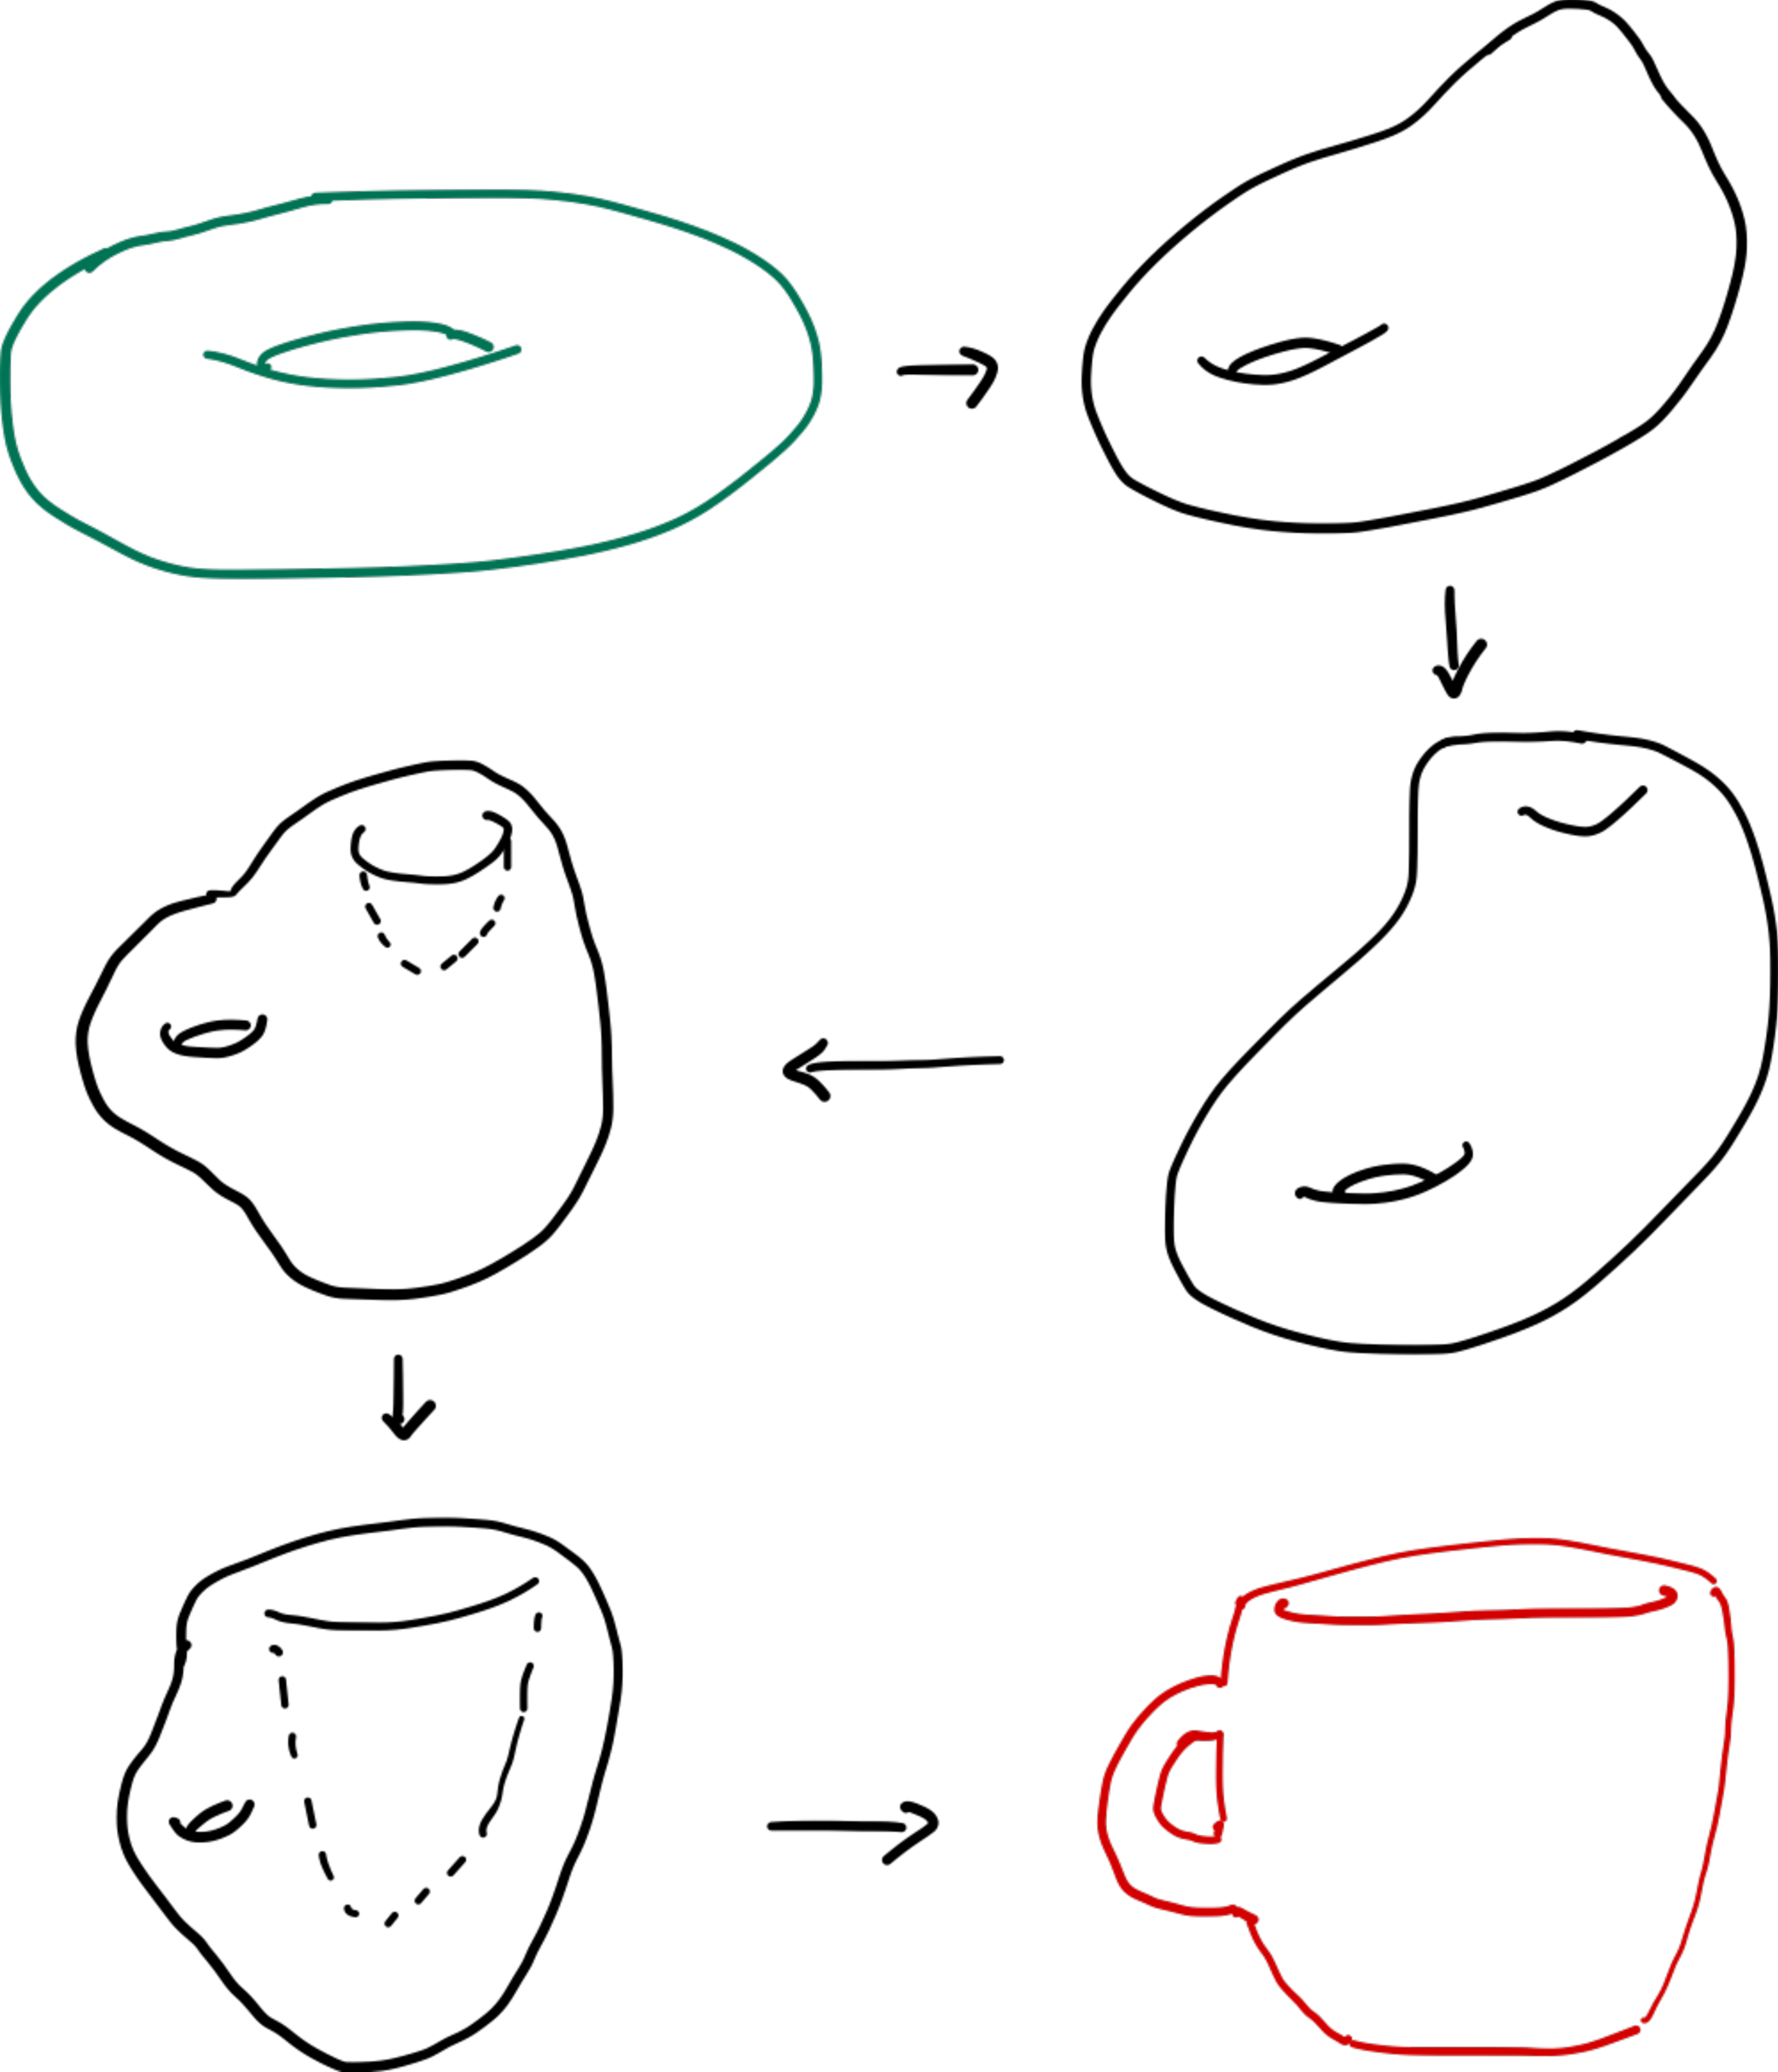
\includegraphics{images/1_1-dount-to-cup.pdf}
  \vspace{5pt}
\end{marginfigure}

\begin{defn}
  A topological space $(X, \cT)$ is \emph{Hausdorff} if every two distinct points admit disjoint open neighborhoods. That is, for every pair $x\neq y$ of points in $X$, there exist open subsets $O_x, O_y\in\cT$ such that $x\in O_x$, $y\in O_y$ and $O_x \cap O_y = \emptyset$.
\end{defn}

Topological spaces are extremely general, as such they may have very inconvenient -- someone would say nasty -- properties.
You can see this for yourself with the following exercise.

\begin{exe}
Let $X$ be an arbitrary set. Show that $\cT:=\{\emptyset, X\}$ defines a topology on $X$, called the \emph{trivial topology}. Show that on $(X, \cT)$ any sequence in $X$ converges to every point of $X$, and every map from a topological space into $X$ is continuous.
\end{exe}

Hausdorff spaces are still rather general: in particular, any metric space with the metric topology\footnote{Recall that in a metric space $X$ the \emph{metric topology} is defined in the following way: a set $U\subset X$ is called open if for any $x\in U$ there exists $\epsilon>0$ such that $U$ fully contains the ball of radius $\epsilon$ around $x$.} is Hausdorff.

\begin{defn}
  A topological space $(X, \cT)$ is \emph{second countable} if there exists a countable set $\cB\subset\cT$ such that any open set can be written as a union of sets in $\cB$.
  In such case, $\cB$ is called a (countable) basis for the topology $\cT$.
\end{defn}

\begin{exe}[Euclidean space $\R^n$]\label{exe:rntopsp}
  Let's consider on $\R^n$ the metric topology\footnote{See comment above.} induced by the Euclidean metric $d: \R^n \times \R^n \to [0, +\infty)$, $d(x,y) := \sqrt{\sum_{i=1}^n (x^i-y^i)^2}$.
  The topological space defined on $\R^n$ is Hausdorff and second countable.
\end{exe}

\begin{defn}[Topological manifold]
  A topological space\footnote{From now on, if we say that $X$ is a topological space we are implying that there is a topology $\cT$ defined on $X$.} $M$ is a \emph{topological manifold} of dimension $n$, or topological $n$-manifold, if it has the following properties
  \begin{enumerate}[(i)]
    \item $M$ is a Hausdorff space;
    \item $M$ is second countable;
    \item $M$ is \emph{locally euclidean} of dimension $n$, \marginnote{This means that any point $x\in M$ has a neighborhood that is homeomorphic to an open subset of $\R^n$.}that is, for any point $x\in M$ there exist an open subset $U\subset M$ with $x\in U$, and open subset $V\in\R^n$ and a homeomorphism $\phi: U\to V$.
  \end{enumerate}
\end{defn}

\begin{ntn}
  Reusing the notation of the definition above, we call \emph{(coordinate) chart} the pair $(U, \phi)$ of a \emph{coordinate neighborhood} $U$ and an associated \emph{coordinate map}\footnote{Or \emph{coordinate system}.} $\phi: U\to V$ onto an open subset $U=\phi(V)\subseteq\R^n$ of $\R^n$.
  Furthermore, we say that a chart is \emph{centered at $m\in U$} if $\phi(m) = 0$.
\end{ntn}

Don't get scared by the first two conditions: they are only needed to make sure that there are not too few open sets (Hausdorff) and not too many (second countable).

\begin{ex}
  With our definition, a countable collections of points with the discrete topology is a $0$-dimensional topological manifolds.
  An uncountable collection of points with the discrete topology, however, is not!
\end{ex}

\begin{ex}
  $\R^n$ is trivially\footnote{Use Exercise \ref{exe:rntopsp} and the \emph{global} chart $(\R^n, \id_{\R^n})$, where $\id_{\R^n}(x) := x$ is the identity on $\R^n$.} a topological manifold of dimension $n$.
  More generally, any $n$-dimensional vector space\footnote{In fact, any subset of a $n$-dimensional vector space.} is a topological $n$-manifold.
\end{ex}

\begin{exe}
	Even though $\R^n$ with the euclidean topology is Hausdorff, being Hausdorff does not follow from being locally euclidean. A famous counterexample is the following\footnote{See also Problem 5.1 in \cite{book:tu}.}.
  \begin{marginfigure}
    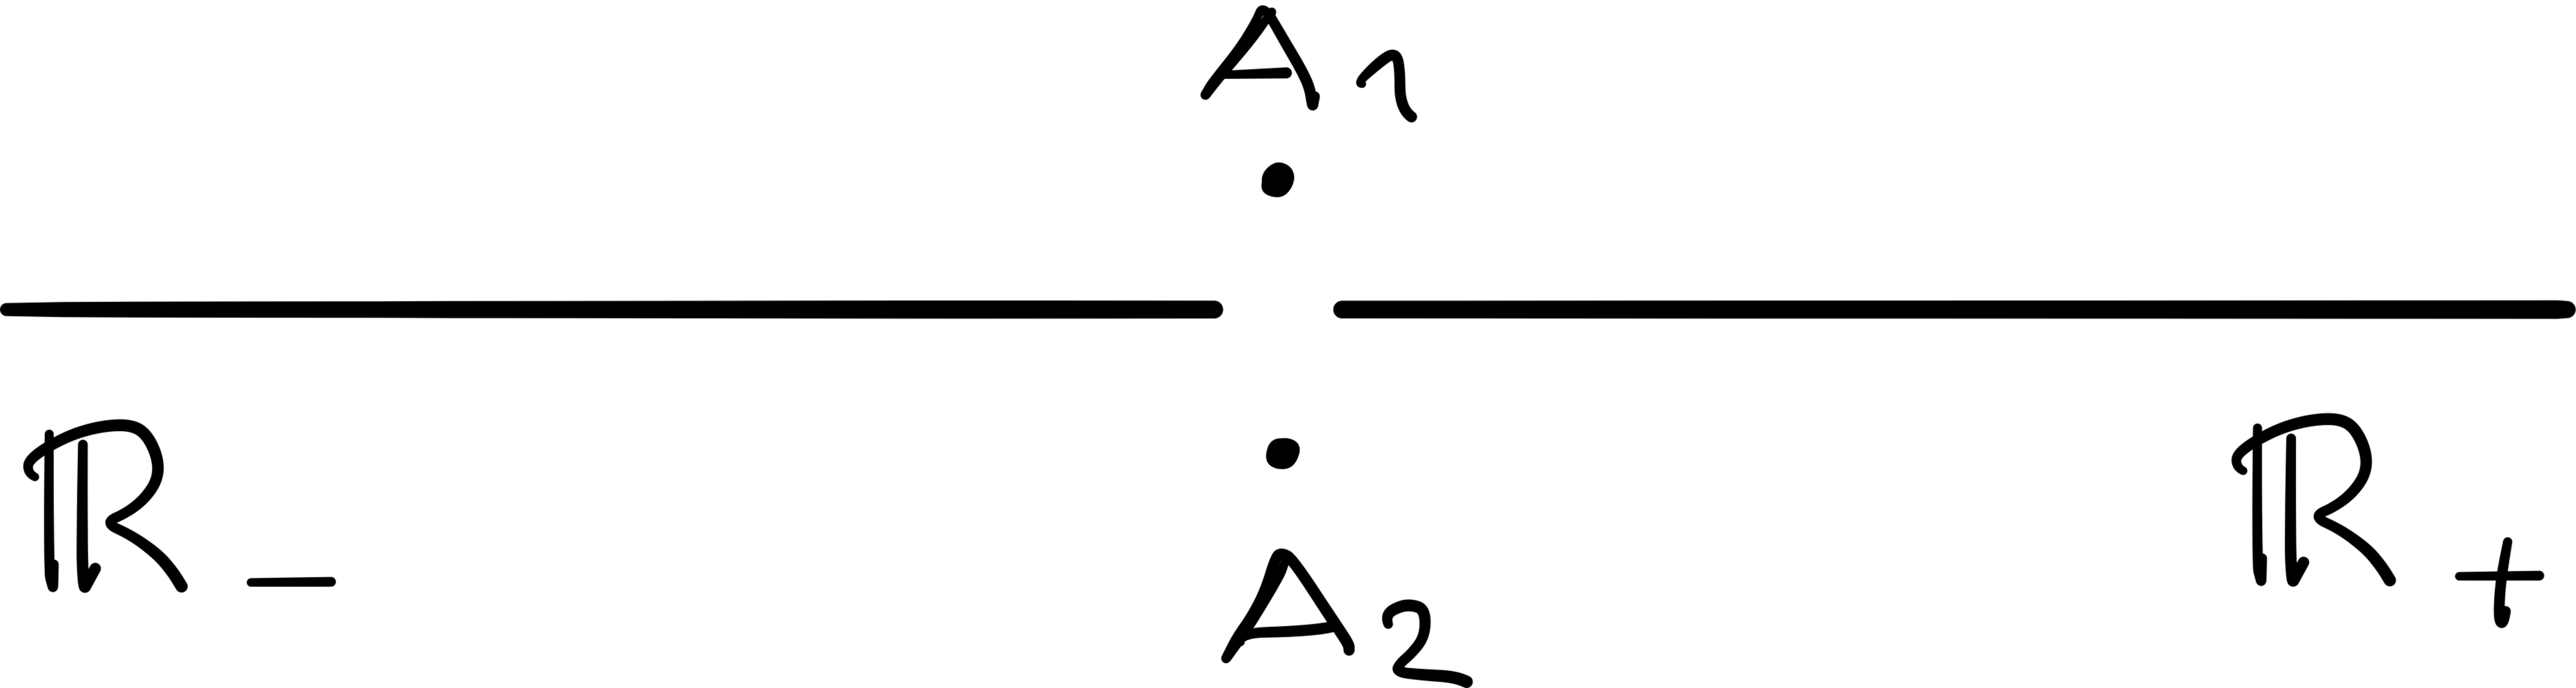
\includegraphics{1_ex_1_0_11.pdf}
    \label{fig:hausdorff-not-locally-euclidean}
    \caption{A locally euclidean space which is not Hausdorff.}
  \end{marginfigure}
  Let $A_1, A_2$ be two point not on the real line $\R$ and define $M:= (\R\setminus\{0\})\cup\{A_1,A_2\}$.
  Define the two charts
  \begin{equation}
  \phi_j:(\R\setminus\{0\})\cup\{A_j\} \to \R, \quad
  \phi_j(x) = \begin{cases} x &\mbox{if } x\neq A_j\\ 0 & \mbox{if } x = A_j \end{cases}, \quad
  j = 1,2.
  \end{equation}
  \begin{enumerate}[(a)]
    \item Show that $\phi_1$ and $\phi_2$ are homeomorphisms with respect to the induced topology\footnote{Let $(X, \cT)$ be a topological space and $f: X\to Y$ some map. The induced topology on $Y$ is \begin{equation}\cU_f := \{f^{-1}(U) \;\mid\; U\in\cT\}.\end{equation}}.
    \item Show that $M$ is locally euclidean and second countable but not Hausdorff.
  \end{enumerate}
\end{exe}

\begin{ex}\label{ex:uball}
  The \emph{closed} unit ball $D_1(0)$, where similarly as before
  \begin{equation}
    D_r(x) := \{z\in\R^n \;\mid\; d(z,x) \leq r\},
  \end{equation}
  is \emph{not} a topological manifold of dimension $n$. Can you see why? In fact, this is an example of a more general concept of \emph{manifold with boundary} that we will introduce later in Chapter~\ref{sec:mbnd}.
\end{ex}

\begin{ex}
	Consider the set $M := \{ x\in\R^2 \;\mid\; |x^1| = |x^2| \}$ with the topology induced by $\R^2$:
   this is \emph{not} a topological manifold.
	Since the number of connected component is invariant under homeomorphisms, open connected neighbourhoods of $(0,0)\in M$ cannot be\footnote{A drawing of $M$ is worth more than a hundred words.} holomorphically mapped to open connected sets in $\R$.
\end{ex}

\marginnote{There is a caveat, the theorem holds for \emph{connected} components of a Manifold. If you consider two distinct connected components, you can indeed have different dimensions for each of them.}
\newthought{There is still an elephant in the room} in need of a comment.
In our definition of topological manifolds, we are giving for granted that the dimension of the manifold is well defined, that is, if we have two different charts, $\phi_1: U \to \R^n$ and $\phi_2: U \to \R^m$, then necessarily $m=n$. Luckily this is true! The result is called \emph{Invariance Domain Theorem} and, since its proof requires advanced concepts of algebraic topology, we will not pursue it further in the course.

\section{Differentiable manifolds}

Before entering into the details of new definitions, let's recall what will be the most important tools throughout the rest of the course.

\begin{defn}
  A map $f: U \to V$ between open sets $U\subset\R^n$ and $V\subset\R^m$ is in $C^r(U,V)$ or \emph{of class $C^r$}, if it is differentiable $r$-times. It is called a $C^r$-diffeomorphism\footnote{With this definition a homeomorphism is a $C^1$-diffeomorphism} if it is bijective and of class $C^r$ with inverse of class $C^r$.
  We say that $f$ is \emph{smooth}\marginnote{To be comprehensive, one should also include $C^\omega$, the class of analytic functions.} or of class $C^\infty$ if it is of class $C^r$ for every $r \geq 1$.
\end{defn}

\begin{thm}[Chain rule]\label{thm:chainrule}
Let $U\subset\R^n$ and $V\subset\R^k$ be open sets and $f: U \to \R^k$, $g: V\to\R^m$ two continuously differentiable functions such that $f(U)\subset V$.
Then, the following holds.
\begin{enumerate}[(i)]
  \item\label{thm:chainrule1} The function $g\circ f: U\subset\R^n \to\R^m$ is continuously differentiable and its total derivative \eqref{eq:jacobian} at a point $x\in U$ is given by
\begin{equation}
  D(g\circ f)(x) = D(g(f(x)) \circ Df(x).
\end{equation}
\item\label{thm:chainrule2} Denote $x=(x^1, \ldots, x^n)\in\R^n$ and $y=(y^2,\ldots,y^k)\in\R^k$ the coordinates on the respective euclidean spaces and $f=(f^1,\ldots,f^k)$ and $g=(g^1,\ldots,g^m)$ the components of the functions. Then the partial derivatives of $g\circ f$ are given by
\begin{equation}
  \frac{\partial g^i\circ f}{\partial x^j}(x)
  = \sum_{r=1}^k \frac{\partial g^i}{\partial y^r}(f(x)) \frac{\partial f^r}{\partial x^j}(x),
\qquad 1\leq i \leq m,\; 1\leq j\leq n.
\end{equation}
\end{enumerate}
\end{thm}

\begin{rmk}
Theorem~\ref{thm:chainrule} has some very deep consequences. First of all \ref{thm:chainrule} \ref{thm:chainrule2} tells us that that composition preserves the regularity, that is the composition of functions  of class $C^r$ is itself a function of class $C^r$.

\marginnote{Follows from the fact that $Df(x)$ is an invertibe matrix and with inverse is $D(f^{-1})(f(x))$.}
Second, if $f:U\subset\R^n\to V\subset\R^m$ is a diffeomorphism, then \ref{thm:chainrule} \ref{thm:chainrule1} implies that $n=m$.
\end{rmk}

Since differentiability is a \emph{local} property and topological manifolds are \emph{locally} like euclidean spaces, it seems reasonable to expect that we can lift the definitions directly from $\R^n$.
If we are given a continuous map between two topological manifolds, we can locally view it as a continuous map between two Euclidean spaces.
Generalizing this further, we could conceivably say that our original map is differentiable if the local map is.

\newthought{As usual, the devil is in the details}: a topological manifold is only homeomorphic to a Euclidean space, and a different choice of homeomorphism might affect whether the local map is differentiable or not.
We need to have extra care to ensure that these lifted definitions keep making sense when we use different charts that overlap.

The solution is to introduce a little more structure to the problem.

\begin{defn}\label{def:crcomp}
We say that two charts $(U_1, \phi_1)$ and $(U_2, \phi_2)$ on a topological manifold $M$ are \emph{$C^r$-compatible} if either $U_1 \cap U_2 = \emptyset$ or if the \emph{transition map}\footnote{Both the composition maps $\phi_1 \circ \phi_2^{-1}$ and $\phi_2 \circ \phi_1^{-1}$ are called transition maps. Both maps are necessarily homeomorphisms since $\phi_1$ and $\phi_2$ are.}
\begin{equation}
  \phi_1 \circ \phi_2^{-1} : \phi_2(U_1\cap U_2) \to \phi_1(U_1 \cap U_2)
\end{equation}
is a diffeomorphism of class $C^r$.
\end{defn}

\begin{figure*}[htp]
  \centering
  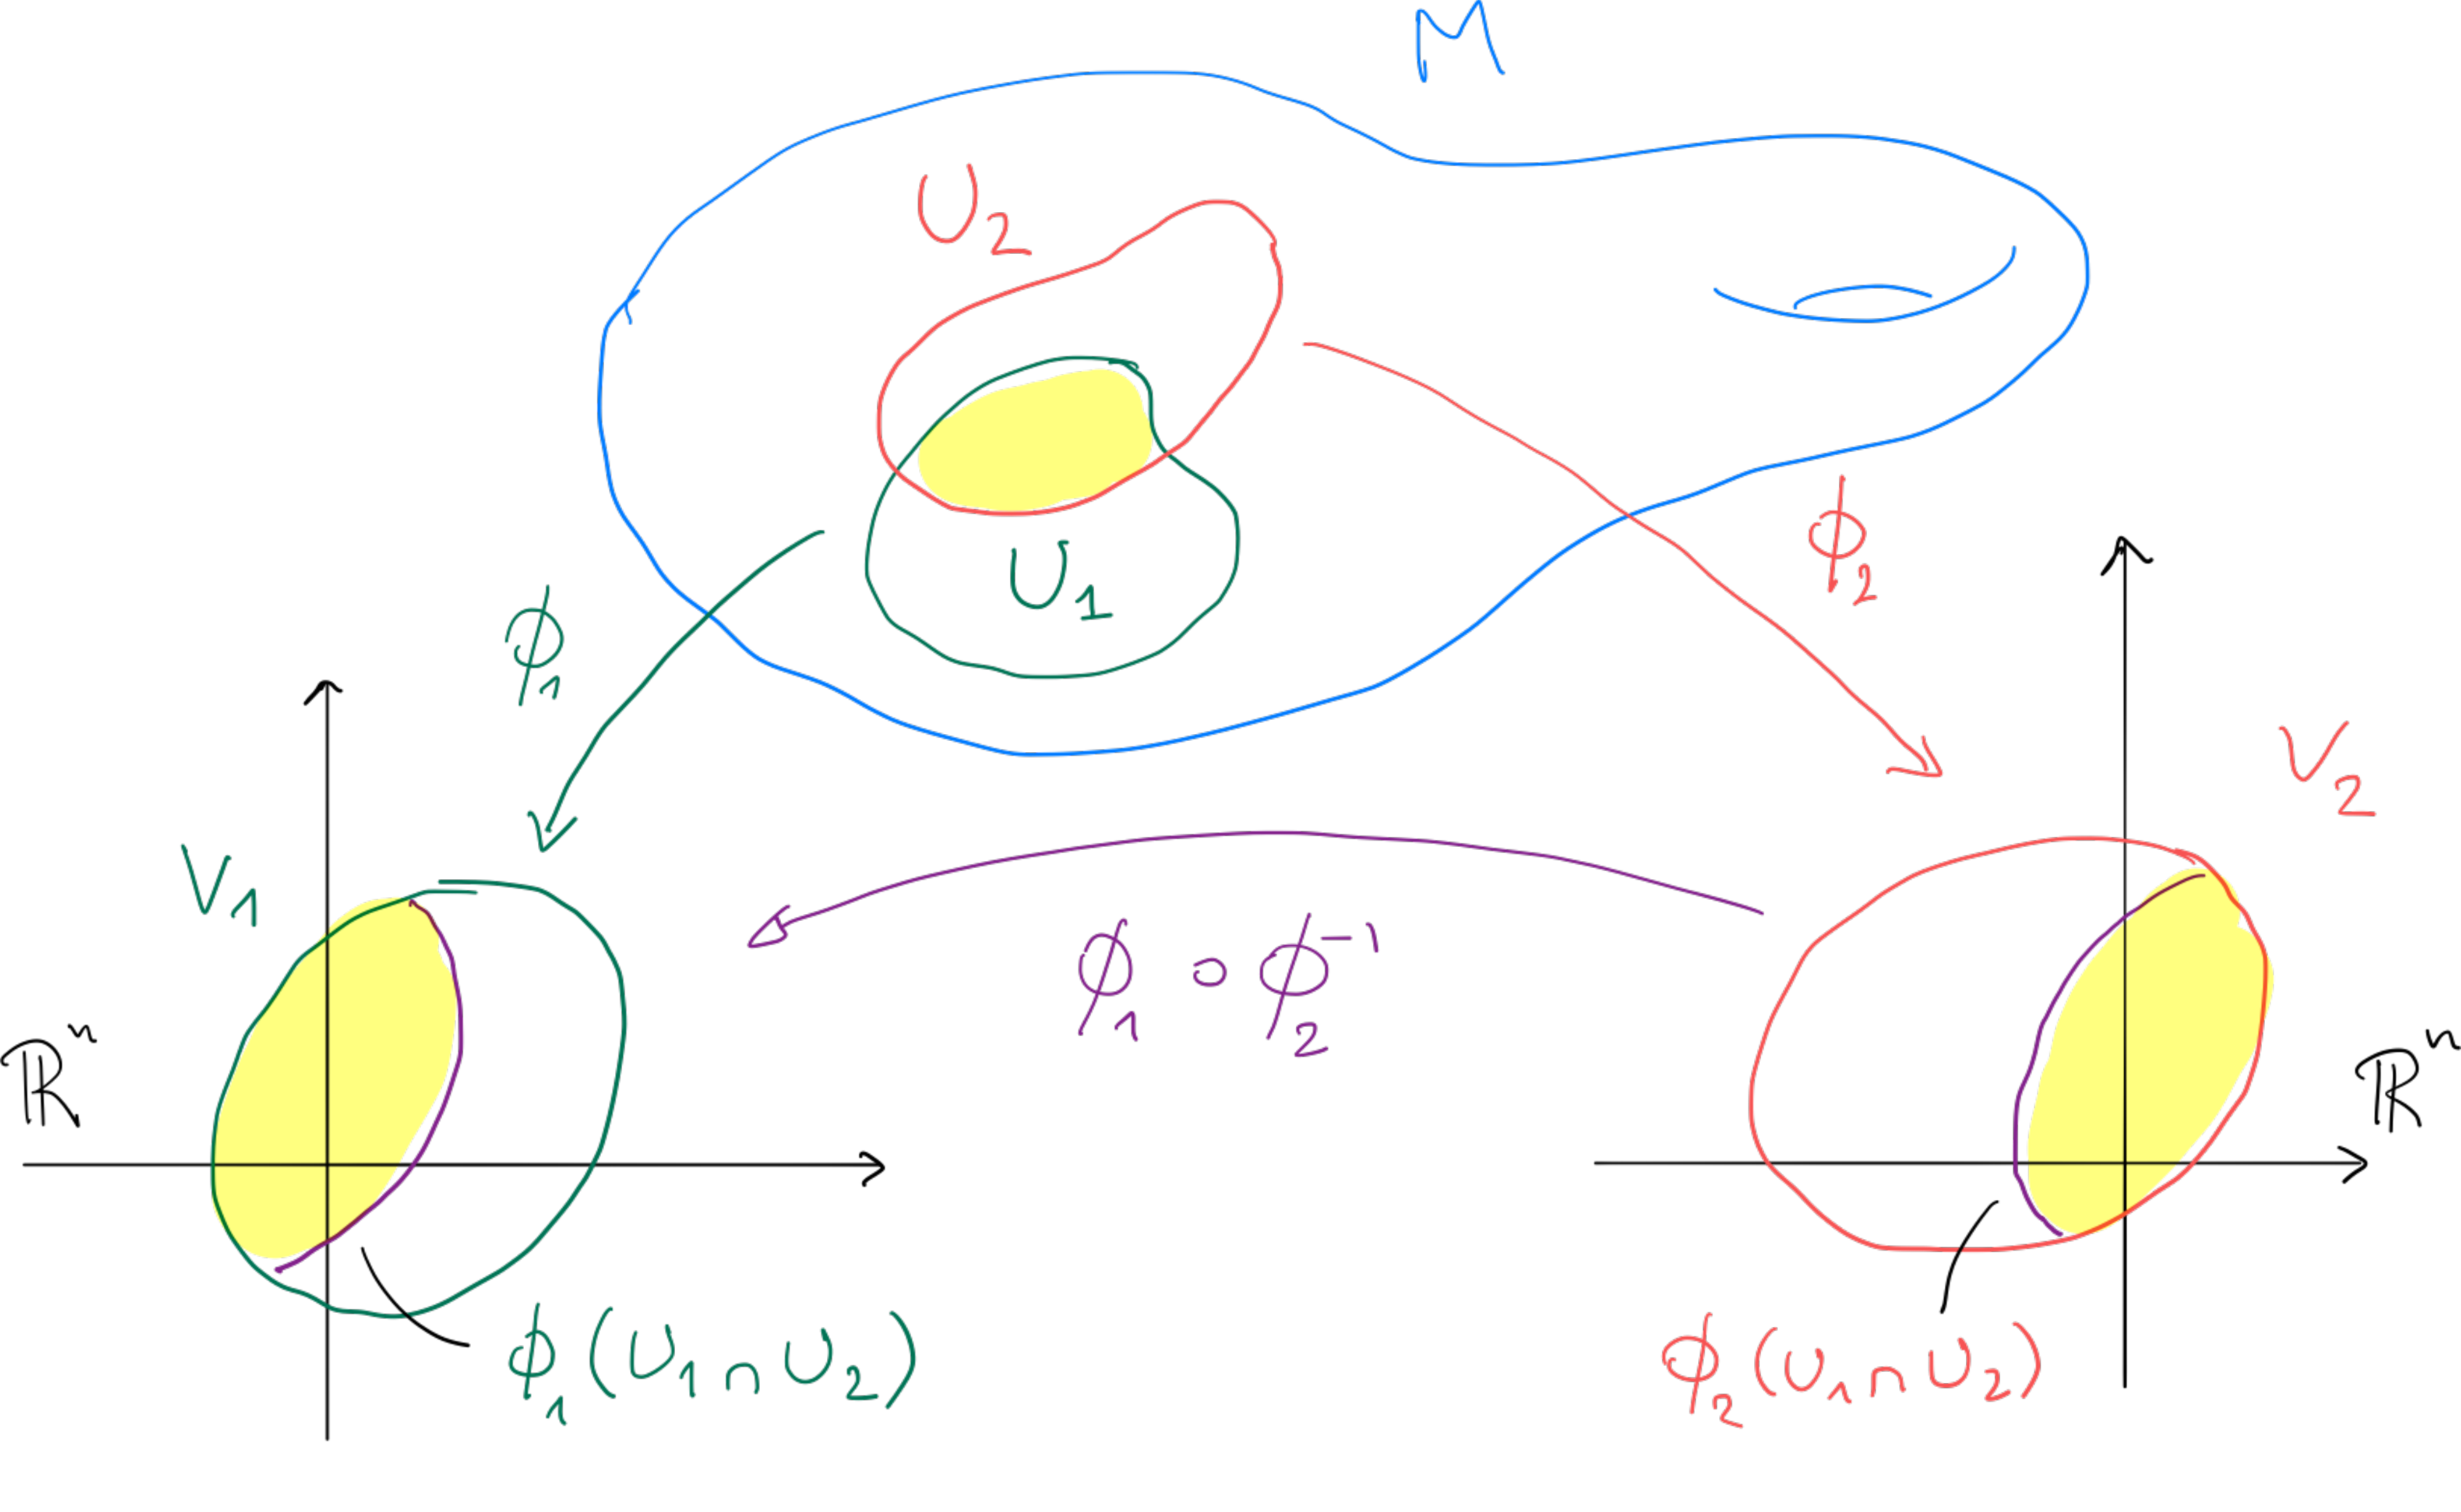
\includegraphics{1_2-compatible-charts.pdf}
  \caption{Charts are compatible if they coincide on the intersections of their coordinate neighborhoods.}
  \label{fig:1.2-compatible-charts}
\end{figure*}

With these at hand, let's jump into the definition of smooth manifolds.

\begin{defn}\label{def:cratlas}
  A \emph{$C^r$-atlas} is a collection
  \begin{equation}
    \cA = \{\phi_\alpha: U_\alpha \to V_\alpha \;\mid\; \alpha\in A\}
  \end{equation}
  of pairwise $C^r$-compatible charts that cover\footnote{I.e. such that $M = \cup_{\alpha\in A} U_\alpha$. One calls the set $\{U_\alpha \;\mid\; \alpha\in A\}$, covering $M$ with open sets, a \emph{open cover} of $M$. Here $A$ is some index set, not necessarily countable.} $M$.

  Two $C^r$-atlases are \emph{equivalent} if their union is also a $C^r$-atlas. That is if any two charts in the atlases are $C^r$-compatible.
\end{defn}

\begin{exe}
  Show that the equivalence of atlases is really an equivalence relation.
\end{exe}

\begin{defn}\label{def:diffstr}
  A \emph{differentiable structure}, or more precisely a \emph{$C^r$-structure}\marginnote[-1.5em]{If $r=\infty$ we simply call it \emph{smooth structure}.}, on a topological manifold is an equivalence class of $C^r$-atlases.
  \marginnote{The union of all atlases in a differentiable structure is the \emph{unique} \emph{maximal} atlas in the equivalence class. There is a one-to-one correspondence between differentiable structures and maximal differentiable atlases: for convenience and to lighten the notation, from now on, we will always regard a differentiable structure as a differentiable maximal atlas without further comments.}
\end{defn}

\begin{defn}\label{def:diffmanifold}
  A \emph{differentiable manifold} of dimension $n$ is a pair $(M, \cA)$ of a topological $n$-manifold $M$ and a differentiable structure $\cA$ on $M$.
  \marginnote[1em]{There are no preferred coordinate charts on a manifold: all coordinate systems compatible with the differentiable structure are on equal footing.}
  A \emph{smooth manifold} of dimension $n$ is a differentiable manifold whose differentiable structure $\cA$ is of class $C^\infty$.
\end{defn}

In colloquial language, a differentiable manifold is a space covered by charts with differentiable transition maps.

Whenever possible we will omit the differentiable structure $\cA$ from the notation and just write $M$.
We may write $M^n$ when we want to emphasize the dimension $n$ of $M$.

\begin{exe}
  Show that on a second countable differentiable manifold it is always possible to find a countable atlas.
\end{exe}

\begin{exe}\label{exe:subsetsmanifolds}
  $\R^n$ with the \emph{standard} smooth structure $\cA=(\R^n, \id_{\R^n})$ is trivially a smooth manifold of dimension $n$.

  In fact, any open subset $U\subset\R^n$ can be made into a smooth manifold in a natural way: pick the atlas $\cA=(U, \id_{\R^n}|_U)$.

  In the same way, any open subset $U$ of a smooth manifold $M$ is a smooth manifold.
  Which atlas would you choose?

  More generally, if $V$ is any $n$-dimensional real vector space, then the standard smooth structure on $V$ is the one induced by the smooth atlas consisting of a single chart $(V, T)$ where $T: V \to R^n$ is some linear isomorphism. Why is this independent of the choice of the isomorphism $T$?

  This example has a very interesting consequence.
  The space $\mathrm{Mat}(n)$ of $n\times n$-matrices can be identified with $\R^{n^2}$ by writing the elements of the matrix as a $n^2$-vector.
  This gives to $\mathrm{Mat}(n)$ a structure of differentiable manifold.
  The subset of invertible matrices $GL(n) = \{ A \in \mathrm{Mat}(n) \;\mid\; \det A \neq 0\}$, widely known as the \emph{general linear group}, being an open subset of $\mathrm{Mat}(n)$ (why?) is itself a differentiable manifold.
Can you guess if such manifold is connected or not?
\end{exe}

\begin{ex}\label{ex:S1emb}
  The unit circle
  \begin{equation}
    \bS^1 := \{x\in\R^2 \;\mid\; \|x\|=1\}\subset\R^2
  \end{equation}
  with the relative topology\footnote{Let $(X,\cT)$ be a topological space and $Y\subset X$. The relative topology on $Y$ is \begin{equation}\mathcal{V}:=\{V\subset Y\;\mid\; V = U \cap Y \mbox{ for some } U\in\cT\}.\end{equation}} is a $1$-dimensional topological manifold.
  To provide the local homeomorphisms to $\R^n$ and define a smooth structure four $\bS^1$ it is enough to define the following four charts:
  \begin{equation}
    \begin{aligned}
      &V_1 := \{ x^1 > 0 \},\quad \phi_1: V_1 \to (-1, 1), \quad \phi_1(x) := x^2,\\
      &V_2 := \{ x^1 < 0 \},\quad \phi_2: V_2 \to (-1, 1), \quad \phi_2(x) := x^2,\\
      &V_3 := \{ x^2 > 0 \},\quad \phi_3: V_3 \to (-1, 1), \quad \phi_3(x) := x^1,\\
      &V_4 := \{ x^2 < 0 \},\quad \phi_4: V_4 \to (-1, 1), \quad \phi_4(x) := x^1.
    \end{aligned}
  \end{equation}
  What do these charts look like?
\end{ex}

\begin{exe}
  Let $f: \R^n \to \R^m$ be a smooth map.
  Show that its graph
  \begin{equation}
    \Gamma_f := \{(x, f(x)) \;\mid\; x\in\R^n\} \subset\R^{n+k}
  \end{equation}
  is a smooth manifold of dimension $n$.
\end{exe}

\begin{ex}
  The definition of smooth manifold does not require $M$ to be embedded into some ambient space as in the examples above.
  In fact, we can define the differentiable manifold $\bS^1$ by equipping the topological quotient space $\R/\Z$ with the two charts
  \begin{equation}\textstyle
    \phi_1 : \R/\Z \setminus\{[0]\} \to (0,1)
    \quad\mbox{and}\quad
    \phi_2 : \R/\Z \setminus\{[\frac12]\} \to (-\frac12,\frac12)
  \end{equation}
  which map $[x]\in\R/\Z$ to its representation in $(0,1)$ or $[-\frac12, \frac12)$ respectively.
  The manifold obtained in this way is diffeomorphic to the one defined in Example \ref{ex:S1emb}.
\end{ex}

\begin{ex}[Product manifolds]
Given two manifolds $(M_1, \cA_1)$ and $(M_2, \cA_2)$, we can define the \emph{product manifold} $M_1 \times M_2$ by equipping $M_1 \times M_2$ with the product topology\footnote{Open sets in the product are products of open sets from the respective topological spaces.} and cover the space with the atlas $\{ (U_1\times U_2, (\phi_1, \phi_2)) \;\mid\; (U_1, \phi_1)\in\cA_1, (U_2, \phi_2)\in \cA_2\}$.
\end{ex}

Note that smooth manifolds do not yet have a metric structure: distances between the points are not defined.
However, they are \emph{metrizable}\footnote{This property is far more general: all the topological manifolds are metrizable.}: there exists some metric on the manifold that induces the given topology on it.
This allows to always view manifolds as metric spaces.

\begin{rmk}
	There exist examples of topological manifolds without smooth structures.
	It is also known that smooth manifolds of dimension $n < 4$ have exactly one smooth structure while ones of dimension $n > 4$ have finitely many\footnote{A beautiful example of this is the $7$-sphere $\bS^7$ which is known to have 28 non-diffeomorphic smooth structures.}.
	The case $n = 4$ is unknown: if you prove that there is only one smooth structure, you will have shown the smooth Poincar\'e conjecture.
\end{rmk}


\subsection{Differentiable maps}

With a well defined differentiable structure and the idea of compatible charts, we have all the ingredients to lift the definition of differentiable maps from the euclidean world.

\begin{defn}
  Let $f:M_1\to M_2$ be a continuous map \footnote{Remember: continuity is not a problem since $M_1$ and $M_2$ are topological spaces.} between two $C^r$-manifolds of dimension $n_1$ and $n_2$ respectively.
  \marginnote[2em]{Differently from your calculus classes, we are defining differentiability \emph{before} we define what the derivative is. Getting to it will require some amount of work, and will have to wait until the next chapter.}
  We say that $f$ is \emph{of class $C^p$}, or \emph{$p$-times differentiable}, ($p \leq r$) if, for any chart $(\phi_1, V_1)$ of $M_1$ and $(\phi_2, V_2)$ of $M_2$, the map
  \begin{align}
    \phi_2 \circ f \circ \phi_1^{-1}: U_1 \to U_2,\\
    U_1 := \phi_1(V_1 \cap f^{-1}(V_2))\subset\R^{n_1},\\
    U_2 := \phi_2(f(V_1) \cap V_2)\subset\R^{n_2},
  \end{align}
  is $p$-times continuously differentiable.
  We denote by $C^p(M_1, M_2)$ the set of all functions $f:M_1\to M_2$ of class $C^p$.

\begin{figure}[htp]
  \centering
  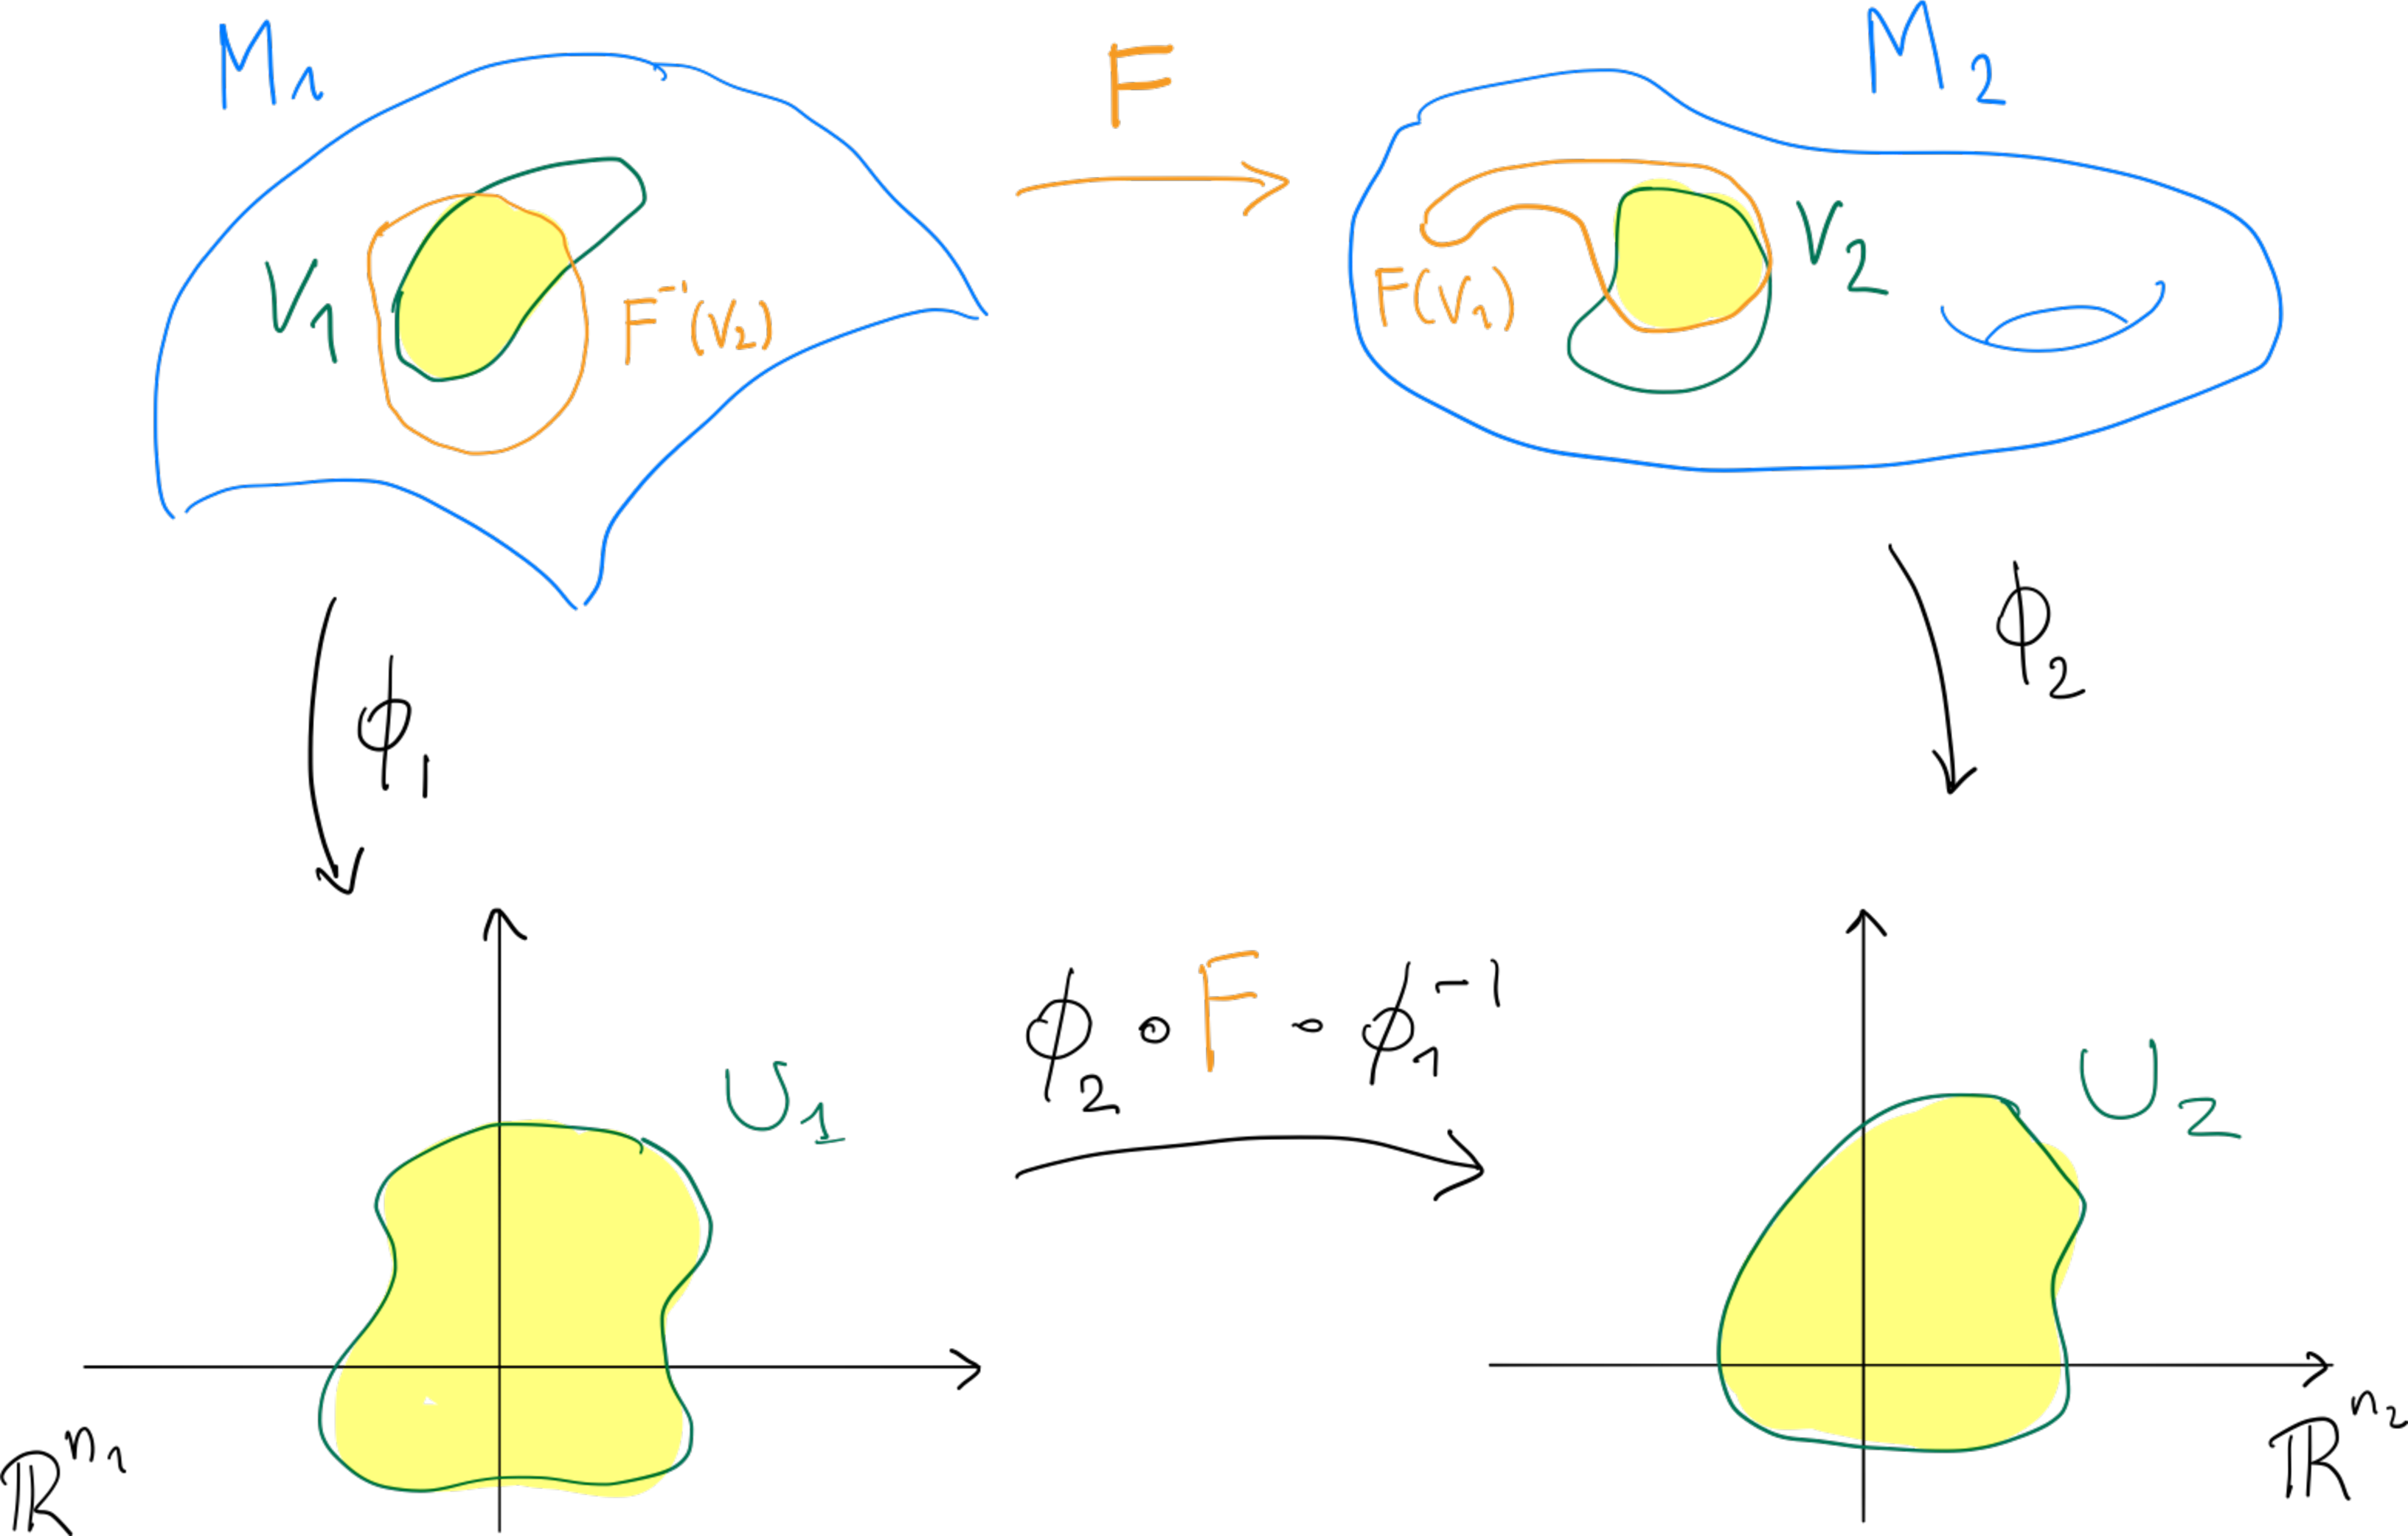
\includegraphics{1_3-diffble_maps.pdf}
  \caption{Maps are differentiable when they are differentiable as maps between euclidean spaces.}
  \label{fig:1.3-differentiable_maps}
\end{figure}

  If $f:M_1\to M_2$ between two smooth manifolds is of class $C^p$ for all $p$, then we say that $f$ is \emph{smooth} or \emph{of class $C^\infty$}.
\end{defn}

\begin{defn}
A \emph{$C^p$-diffeomorphism} $f$ between two $C^r$-manifolds $M_1$ and $M_2$, $p \leq r$, is a bijective map such that $f\in C^p(M_1, M_2)$ and $f^{-1}\in C^p(M_2, M_1)$.

If $f:M_1\to M_2$ between two smooth manifolds $M_1$ and $M_2$ is a $C^p$-diffeomorphism for all $p$, then we say that $f$ is a \emph{diffeomorphism}.
Two smooth manifolds $M_1$ and $M_2$ are called \emph{diffeomporphic} if there exists a diffeomorphism $f:M_1\to M_2$ between them.
\end{defn}

\begin{ex}
Any chart $(V, \phi)$ of a manifold $M$ is a diffeomorphism between the manifolds $V\subset M$ and $\phi(V)\subset\R^n$.
\end{ex}

\begin{exe}
  Prove the following propositions and aid your reasoning by drawing the relevant figures.
  \begin{prop}
    Let $M$ be a $C^r$-manifold of dimension $n$.
    Then $f:M\to\R^m$ is of class $C^r$ iff for all charts $(U,\phi)$ of $M$, the function $f\circ\phi^{-1}:\phi(U)\to\R^m$ is of class $C^r$.
  \end{prop}
  \begin{prop}
    Let $M$ be a $C^r$-manifold of dimension $n$.
    Then $f:\R^m\to M$ is of class $C^r$ iff for all charts $(U,\phi)$ of $M$, the function $\phi\circ f:f^{-1}(U)\to\R^m$ is of class $C^r$.
  \end{prop}
  \begin{prop}
    Let $M, N, P$ be three $C^r$-manifolds, and suppose that $f:M\to N$ and $g:N\to P$ are of class $C^r$.
    Then $g\circ f\in C^r(M, P)$.
  \end{prop}
  \marginnote{In Proposition~\ref{prop:uniqdiffeoinclusion} it is not enough to ask that $\iota$ is smooth! As counterexample consider the two manifolds $(\R, \cA_1)$ with $\cA_1 := \{(\R, \id_\R)\}$ and $(\R, \cA_2)$ with $\cA_2 := \{(\R, x\mapsto x^3)\}$. The inclusion of open sets in $\R$ is smooth in both cases but is a diffeomorphism only in one.}
  \begin{prop}\label{prop:uniqdiffeoinclusion}
    Let $M$ be a manifold and $U\subset M$ an open set.
    Then $U$ has a unique differentiable structure such that the inclusion $\iota:U\hookrightarrow M$ is a diffeomorphism.
  \end{prop}
  \begin{prop}[Smoothness is a local property]\label{prop:smoothlocal}
    Let $f:M\to N$ be a continuous function and let $\{U_i\}_{i\in I}$ be an open cover for $M$. Then $f|_{U_i}:U_i \to N$ is smooth for every $i\in I$ iff $f:M\to N$ is smooth.
  \end{prop}
\end{exe}

\subsection{Manifolds with boundary}\label{sec:mbnd}

\newthought{The definition of manifolds has a serious limitation}, even though it is perfectly good to describe curves\footnote{E.g. the circle seen in Example~\ref{ex:S1emb}.} and surfaces\footnote{E.g. the $n$-spheres $\bS^n$ in the homework sheet.}, it fails to describe many natural objects like a \emph{closed} interval $[a,b]\in\R$ or the \emph{closed} disk $D_1(0)$ of Example~\ref{ex:uball}.

Note that in both these cases, both the interior and the boundary are smooth manifolds and their dimension differ by one\footnote{In the first case the interior $(a,b)$ is a $1$-manifold and the boundary, the set $\partial[a,b] = \{a,b\}$, is a $0$-manifold. In the second case the interior of $D_1(0)$ is the open unit ball, a $2$-manifold, and the boundary $\partial D_1(0)$ is the $1$-manifold $\bS^1$.}.

Let's do a step back and think about topological manifolds: since both the closed interval and the closed disk are closed sets, we have problems to make them locally euclidean in neighbourhoods of their boundaries.
Can we modify our local model to resemble something with a boundary?

\begin{marginfigure}
  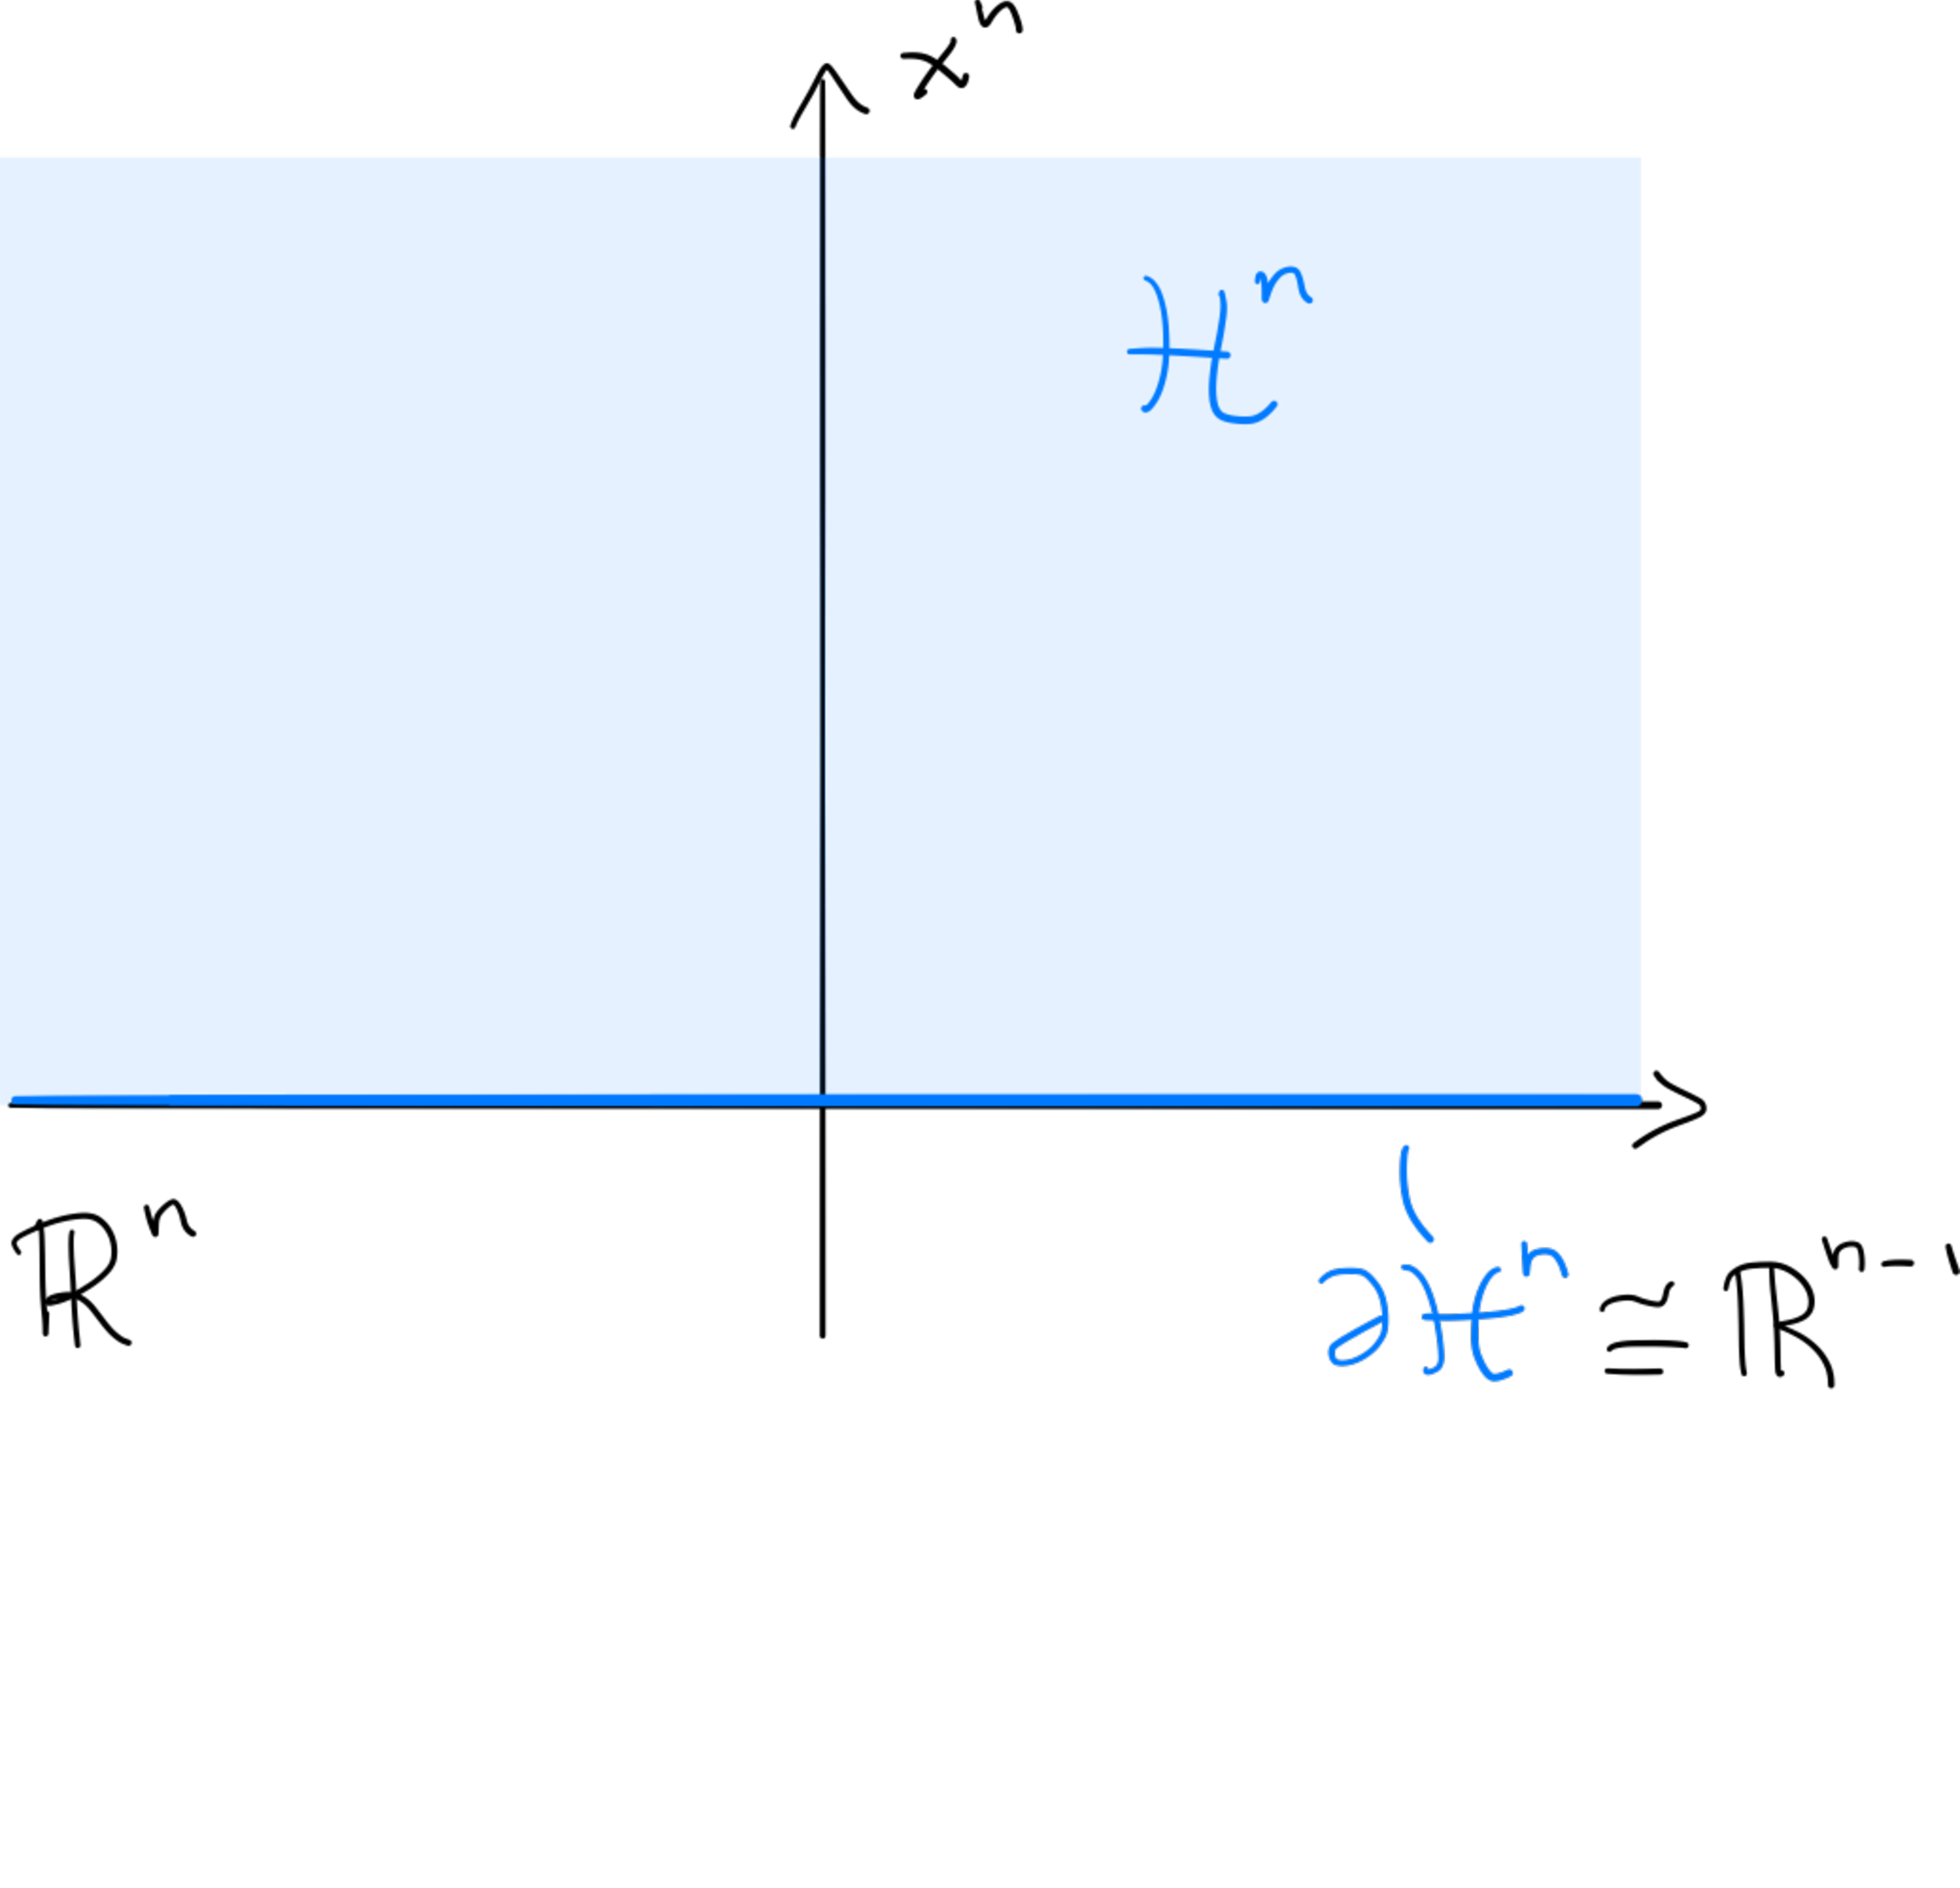
\includegraphics{1_4-upper_space.pdf}
\end{marginfigure}
Of course this is a rhetorical question.
We can generalize our definition by considering the \emph{closed upper half-spaces}
\begin{equation}
  \cH^n = \R_+^n = \{x=(x^1, \ldots, x^n)\in\R^n\mid x^n \geq 0\},
\end{equation}
with its $(n-1)$-dimensional boundary
\begin{equation}
  \partial\cH^n = \{x=(x^1, \ldots, x^n)\in\R^n\mid x^n = 0\}
\end{equation}
and the topology inherited by $\R^n$, as a replacement for our local model $\R^n$.

\begin{defn}
  A topological space $M$ is a \emph{topological manifold with boundary} of dimension $n$, or topological $n$-manifold with boundary, if it has the following properties
  \begin{enumerate}[(i)]
    \item $M$ is a Hausdorff space;
    \item $M$ is second countable;
    \item $M$ is \emph{locally} homeomorphic to $\cH^n$, any point $x\in M$ has a neighborhood that is homeomorphic to a (relatively) open\footnote{Recall that $U\subset\R^n_+$ is relatively open, that is open with respect to the relative topology, if there exist an open set $\tilde U\subset\R^n$ such that $U = \tilde U \cap \R^n_+$.} subset of $\R^n_+$.
  \end{enumerate}

  A \emph{chart} on $M$ is a pair $(U, \phi)$ consisting of an open set $U\subset M$ and a homeomorphism $\phi: U \to \phi(U)\subset \cH^n$.
\end{defn}

TODO\todo{add picture}

We saw in Proposition~\ref{prop:uniqdiffeoinclusion} that differentiability\footnote{In fact, also $C^r$-differentiability} is a local property, which means that is a property defined on open sets.
To clarify what it means to have differentiable structures on manifolds with boundary, we will thus need to clarify what it means for a function defined on $\cH^n$ to be differentiable at points on $\partial\cH^n$.
As it turns out, this is a minor modification of our previous definition that stems directly from the definition of the induced topology.

\begin{defn}
  Let $U\subset\cH^n$ be a relatively open set. A map $f: U\to\R^m$ is \emph{$r$-times continuously differentiable} if there exists an open set $\tilde U\in\R^n$ and a map $\tilde f\in C^r(\tilde U, \R^m)$ such that $U\subset\tilde U$ and $\tilde f|_U = f$.
\end{defn}

With such definition at hand, one can define $C^r$-compatibility, $C^r$-atlases and differentiable structures as in Definition~\ref{def:crcomp}, Definition~\ref{def:cratlas} and Definition~\ref{def:diffstr} by considering charts taking value in $\cH^n$.

\begin{defn}\label{def:diffmanifoldwb}
  A \emph{$C^r$ manifold with boundary} of dimension $n$ is a pair $(M, \cA)$ of a topological $n$-manifold with boundary $M$ and a differentiable structure $\cA = \{(U_\alpha, \phi_\alpha) \mid \alpha\in A\}$ on $M$ of class $C^r$.
  
  The \emph{boundary} of $M$ is defined as
  \begin{equation}
    \partial M := \bigcup_{\alpha\in A} \phi_\alpha^{-1}\left(\phi_\alpha(V_\alpha)\cap \partial\cH^n\right).
  \end{equation}

  A \emph{smooth manifold} of dimension $n$ is a differentiable manifold whose differentiable structure $\cA$ is of class $C^\infty$.
\end{defn}

\begin{prop}
  The boundary $\partial M$ is well defined\footnote{The same definition holds for topological manifolds, but showing that it is well defined is much more complicated and will be omitted.}.
\end{prop}
\begin{proof}
  
\end{proof}

\begin{fullwidth}
Even if we gave the general definition of $C^r$-manifolds, in these notes will be only interested in smooth manifolds.
From now on we always talk about smooth manifolds unless differently specified.

Differentiable manifolds (without boundary)\footnote{See  Definition~\ref{def:diffmanifold}.} can be seen as a special case of differentiable manifolds with boundary\footnote{See Definition~\ref{def:diffmanifoldwb}} where the boundary happens to be empty. Therefore, with the exception of the beginning of Chapter~\ref{ch:2}, we will no-longer distinguish the two concepts: from now on, a manifold may have or may not have a boundary.
\end{fullwidth}

\subsection{Infinite dimensional manifolds $\star$}
TODO\todo{See Merry, Remark 1.31.}

\chapter{Tangent bundle}\label{ch:2}

\chapter{Cotangent bundle}

\chapter{Vector fields}

\chapter{Tensor products}

\chapter{Differential Forms}

\subsection{de Rahm cohomology}

\chapter{Integration of forms}
\subsection{Orientation}

\subsection{Stokes' Theorem}

\begin{appendices}
  \chapter{Solution to selected exercises}
  \section{Chapter \ref{ch:manifolds}}
  
  \newthought{Exercise \ref{exe:rntopsp}.}
  \begin{enumerate}
    \item[] Hausdorff. For $x\neq y\in\R^n$, let $\epsilon = d(x,y)/3$.
    Then the two balls $B_x(\epsilon) := \{z\in X \;\mid\; d(z,x)<\epsilon\}$ and $B_y(\epsilon)$ are disjoint open sets containing $x$ and $y$ respectively.
    \item[] Second countable. As countable basis for the topology we can take the open balls $B_\epsilon(x)$ with rational radii $\epsilon\in\Q$ and centers $x\in\Q^n$.
  \end{enumerate}
  
\end{appendices}

\bibliographystyle{plainnat}
\bibliography{aom}
\addcontentsline{toc}{chapter}{Bibliography}
\end{document}